\section{Directed Graphical Models}
Directed Graphical Models, also known as Bayesian Networks. The joint distribution of a graph with $K$ nodes is given by:
\begin{equation}
    p(x) = \prod_{k=1}^K p(x_k|pa_k)
\end{equation}
where $pa_k$ denotes the set of parents of $x_k$. This is the \textbf{factorization} of a directed graphical model. The learning task is, how to derive join probability distributions to answer questions.

\begin{figure}[tb]
 \centering 
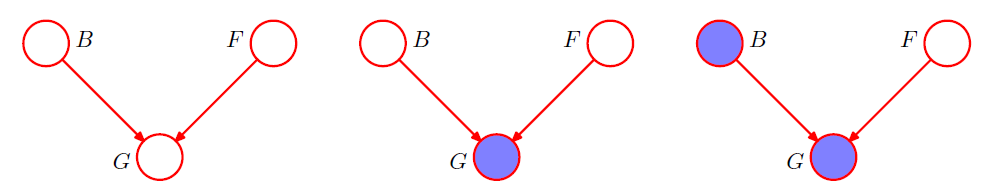
\includegraphics[scale=0.42]{images/DGM.png} 
 \caption{An example of a 3-node graph used to illustrate the phenomenon of ‘explaining away’. The three
nodes represent the state of the battery (B), the state of the fuel tank (F) and the reading on the electric fuel
gauge (G).}
 \label{fig:GDM}
\end{figure}
\textbf{When I turn on the car:} \\
p(B): battery is charged (B=\{0,1\})\\
p(F): there is fuel in the tank (F=\{0,1\})\\
p(G): fuel gauge moves (G=\{0,1\})\\
\\
p(G = 1|B-=1,F=1) = 0.8 \\
p(G = 1|B-=1,F=0) = 0.2 \\
p(G = 1|B-=0,F=1) = 0.2 \\
p(G = 1|B-=0,F=0) = 0.1 \\
p(B=1) = 0.9 \\
p(F=1) = 0.9 \\
From this we can derive: \\
p(G = 0|B-=1,F=1) = 0.2 \\
p(G = 0|B-=1,F=0) = 0.8 \\
p(G = 0|B-=0,F=1) = 0.8 \\
p(G = 0|B-=0,F=0) = 0.9 \\
p(B=0) = 0.1 \\
p(F=0) = 0.1 \\
\textbf{If the gauge does not move, what is the probability that the fuel tank is empty?} \\
\begin{align*}
p(F=0|G=0) & =\frac{p(G=0|F=0)p(F=0)}{p(G=0)} \\
    p(G=0|F=0) & = \sum_{B\in \{0,1\}} p(G=0|B,F=0)p(B) \\
    For B=0: \\
    & = p(G=0|B=0,F=0)p(B=0) \\    
    & = 0.9 * 0.1 \\
    & = 0.09 \\
    For B=1: \\
    &= p(G=0|B=1,F=0)p(B=1) \\   
    & = 0.8 * 0.9 \\
    & = 0.72 \\
p(G=0|F=0) & = 0.09 + 0.72 = \textbf{0.81} \\  
p(F=0) & = \textbf{0.1} \\
p(G=0) & =  \sum_{B\in \{0,1\}}  \sum_{F\in \{0,1\}}  p(G=0|B,F)  p(B)  p(F) \\ 
For B=0, F=0: \\
     & = p(G=0|B=0,F=0)  p(B=0)  p(F=0) \\
    &= 0.9 * 0.1 * 0.1 \\
    & = 0.009 \\
For B=0, F=1: \\
     & = p(G=0|B=0,F=1)  p(B=0)  p(F=1) \\
    &= 0.8 * 0.1 * 0.9 \\
    & = 0.072 \\
For B=1, F=0: \\
     & = p(G=0|B=1,F=0)  p(B=1)  p(F=0) \\
    &= 0.8 * 0.9 * 0.1 \\
    & = 0.072 \\ 
For B=1, F=1: \\
     & = p(G=0|B=1,F=1)  p(B=1)  p(F=1) \\
    &= 0.2 * 0.9 * 0.9 \\
    & = 0.162 \\    
p(G=0) &= 0.009 + 0.072 + 0.072 + 0.162 = \textbf{0.315} \\
p(F=0|G=0) & =\frac{0.81*0.1}{0.315} \\
p(F=0|G=0) & \simeq \textbf{0.257} \\
\end{align*}
Next suppose that we also check the state of the battery and find that it is flat, i.e.,
$B = 0$. The posterior probability that the fuel tank is empty given the observations of both the fuel gauge and the battery state is then given by:
\begin{align*}
    p(F=0|G=0,B=0) = \frac{p(G=0|B=0,F=0)p(B=0)p(F=0)}{\sum_{F\in \{0,1\}p(G=0|B=0,F)p(B=0)p(F)}}
\end{align*}
When expanding the denominator summation, p(B=0) can be factored out and cancelled:
\begin{align*}
    \frac{p(G=0|B=0,F=0)p(B=0)p(F=0)}
    {\big(p(G=0|B=0,F=0)p(F=0) + p(G=0|B=0,F=1)p(F=1)\big)p(B=0)} \\
    \frac{p(G=0|B=0,F=0)p(F=0)}
    {p(G=0|B=0,F=0)p(F=0) + p(G=0|B=0,F=1)p(F=1)}    
\end{align*}
then solved
\begin{align*}
    For F=0: \\
    & = p(G=0|B=0,F=0)p(F=0) \\    
    & = 0.9 * 0.1 \\
    & = 0.09 \\
    For F=1: \\
    & = p(G=0|B=0,F=1)p(F=1) \\    
    & = 0.8 * 0.9 \\
    & = 0.72 \\  
    & = \textbf{0.81} \\      
    p(F=0|G=0,B=0) & = \frac{0.9*0.1}{0.81} \\
    & \simeq \textbf{0.111} 
\end{align*}
In the case of a Naive Bayes Classifier (as a DGM), we again make the assumption of independence:
$$
p(y,\mathrm{x}) = p(y)\prod_{j=1}^Dp(x_j|y)
$$
and would represent the graph likesuch:
\begin{figure}[tb]
 \centering 
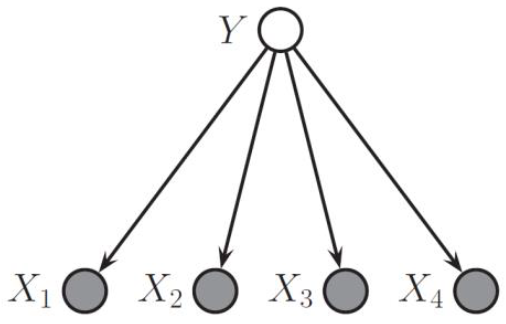
\includegraphics[scale=0.42]{images/bayes-dgm.png} 
 \caption{DGMs - the naive case}
 \label{fig:GDM}
\end{figure}